\section{Documentation and comments}
Most of the functions have a simple comment description, not heavily technical. Everything can be collected and formed into nice-looking documentation using \textit{Haddoc}.
\begin{figure}[H]
  \centering
     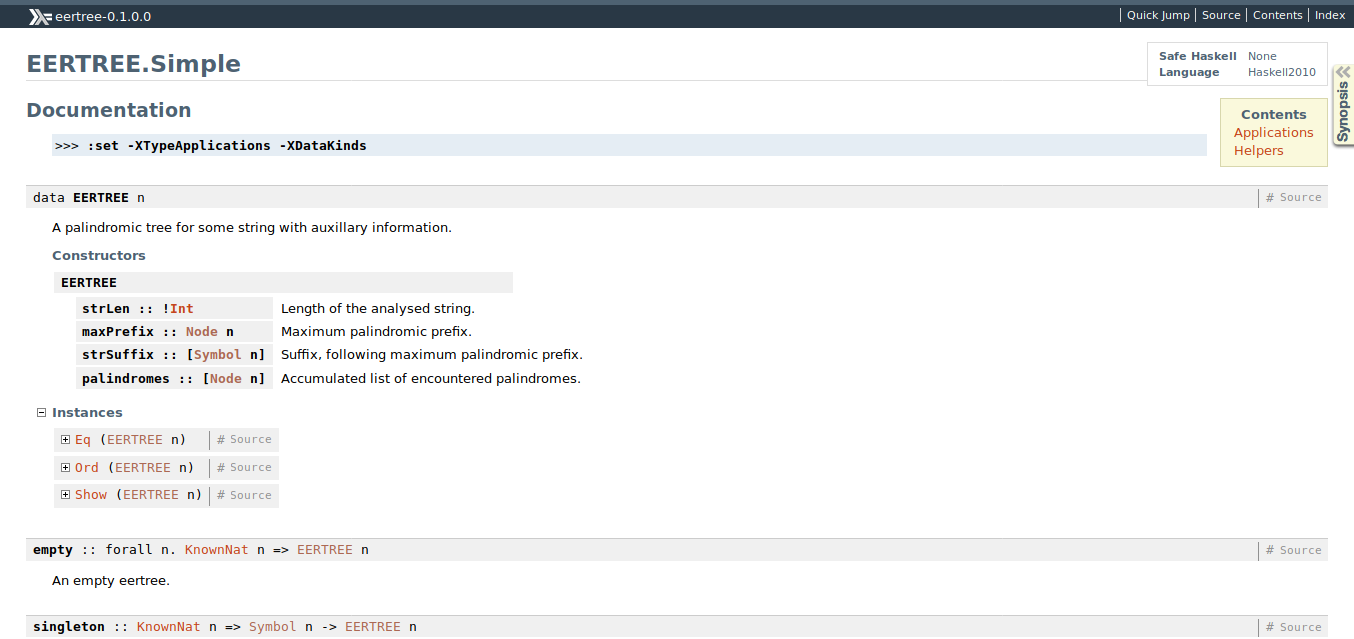
\includegraphics[width=\linewidth]{haddoc.png}
 \caption{Example of some entry generated by haddoc}
\end{figure}
\section{Tests and examples}
Some functions have an example which also can be used as a \textit{doctest}.
\begin{figure}[H]
  \centering
     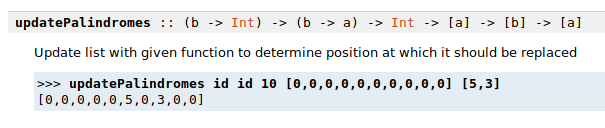
\includegraphics[width=\linewidth]{doctest.png}
 \caption{Example of some entry with doctest}
\end{figure}
\vfill\eject
More complex functions are covered with \textit{QuickCheck's properties}.
\begin{figure}[H]
  \centering
     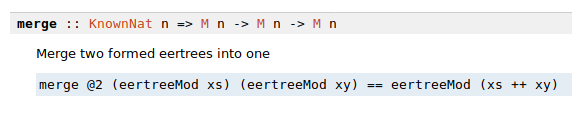
\includegraphics[width=\linewidth]{prop.png}
 \caption{Example of some entry with property test}
\end{figure}





In this example it can be seen as:
$$merge(eertree(S_1), eertree(S_2)) \equiv eertree(S_1 + S_2) $$